
\documentclass{article}

\title{Informe conciso}
\author {Maria Isabel Gamez Salazar}
\date {25 Julio 2024}

\usepackage{hyperref}
\usepackage{geometry}
 \geometry{
 a4paper,
 total={170mm, 257mm},
 left=20mm,
 top=20mm
 }
\renewcommand{\refname}{Referencias}
\renewcommand{\tablename}{Tabla}

\usepackage{Sweave}
\begin{document}
\Sconcordance{concordance:informefinal.tex:informefinal.Rnw:1 18 1 1 0 4 1 1 9 63 1 1 %
26 5 1 1 61 3 1 1 18 3 1 1 22 21 1}

\maketitle
\section {Introducción}


\noindent El presente informe aborda de manera sencilla el nivel de felicidad en la población de 15 países europeos durante el período comprendido entre 2002 y 2014. El análisis tiene como objetivo principal investigar las tendencias y variaciones en la felicidad a lo largo del tiempo, así como identificar posibles factores que puedan influir en este sentimiento.


Los datos se han obtenido a partir de los resultados de 114473 encuestas de las 4 ediciones de la [European Social Survey](https://www.europeansocialsurvey.org/) en 15 países de Europa. Estas encuestas han tenido lugar desde 2002 hasta 2014.


Se espera que este informe proporcione una visión integral sobre los niveles de felicidad en Europa y cómo estos han cambiado a lo largo del tiempo. También se anticipa identificar factores que influyen significativamente en la felicidad, lo cual puede tener implicaciones importantes para la formulación de políticas públicas y estrategias de bienestar social.


Respecto a las variables hay que indicar que:
\begin{itemize}
\item Los valores del nivel de felicidad del encuestado en una escala van del 0 extremadamente infeliz a 10, extremadamente feliz. 
\item Año de la encuesta
\item País dónde se respondió la encuesta.
\end{itemize}

Además de esas, se creará un dashboard en el que se incluirán las siguientes variables para ver si afectan a los resultados:

\begin{itemize}

\item Los valores de las otras variables como el tiempo total de visualización de televisión en un día de semana. El valor de 0 indica "No time at all", 1 significa "Less than 0.5 hour", 2 corresponde a "0.5 hour to 1 hour", 3 representa "More than 1 hour, up to 1.5 hours", 4 es "More than 1.5 hours, up to 2 hours", 5 indica "More than 2 hours, up to 2.5 hours", 6 es "More than 2.5 hours, up to 3 hours", y finalmente, 7 equivale a "More than 3 hours".

\item Los valores de la salud general subjetiva del encuestado van desde 1 corresponde a "Very good", indicando la evaluación más positiva; … y el valor 5 es "Very bad".

\item Los valores para género del encuestado son tradicionales y corresponden al masculino (1), femenino (2), o no responde.

\end{itemize}

\section {Resultados}

\subsection{Tablas}

\begin {tabular}{l | c }
  

\hline
\bf{País} & \bf{Felicidad} \\ 
\hline
BE &	7.750140 \\		
CH &	8.046004 \\		
DE &	7.287895 \\		
DK &	8.291183 \\	
ES &	7.487663 \\	
FI &	8.011595 \\			
FR &	7.161961 \\			
GB &	7.459976 \\			
HU &	6.342159 \\			
IE &	7.359424 \\			
NL &	7.752350 \\			
NO &	7.945898 \\			
PL &	6.949639 \\			
PT &	6.642746 \\			
SE &	7.896336 \\			
\hline
\end{tabular}
\\	
\vspace{0.5cm}
\vspace{0.5cm}

En la tabla superior podemos observar la media de la felicidad de esos años escogidos (2002, 2006, 2010, 2014) para los 15 países seleccionados. 

\subsection {Gráficos}
\begin{figure}[h!]
\centering
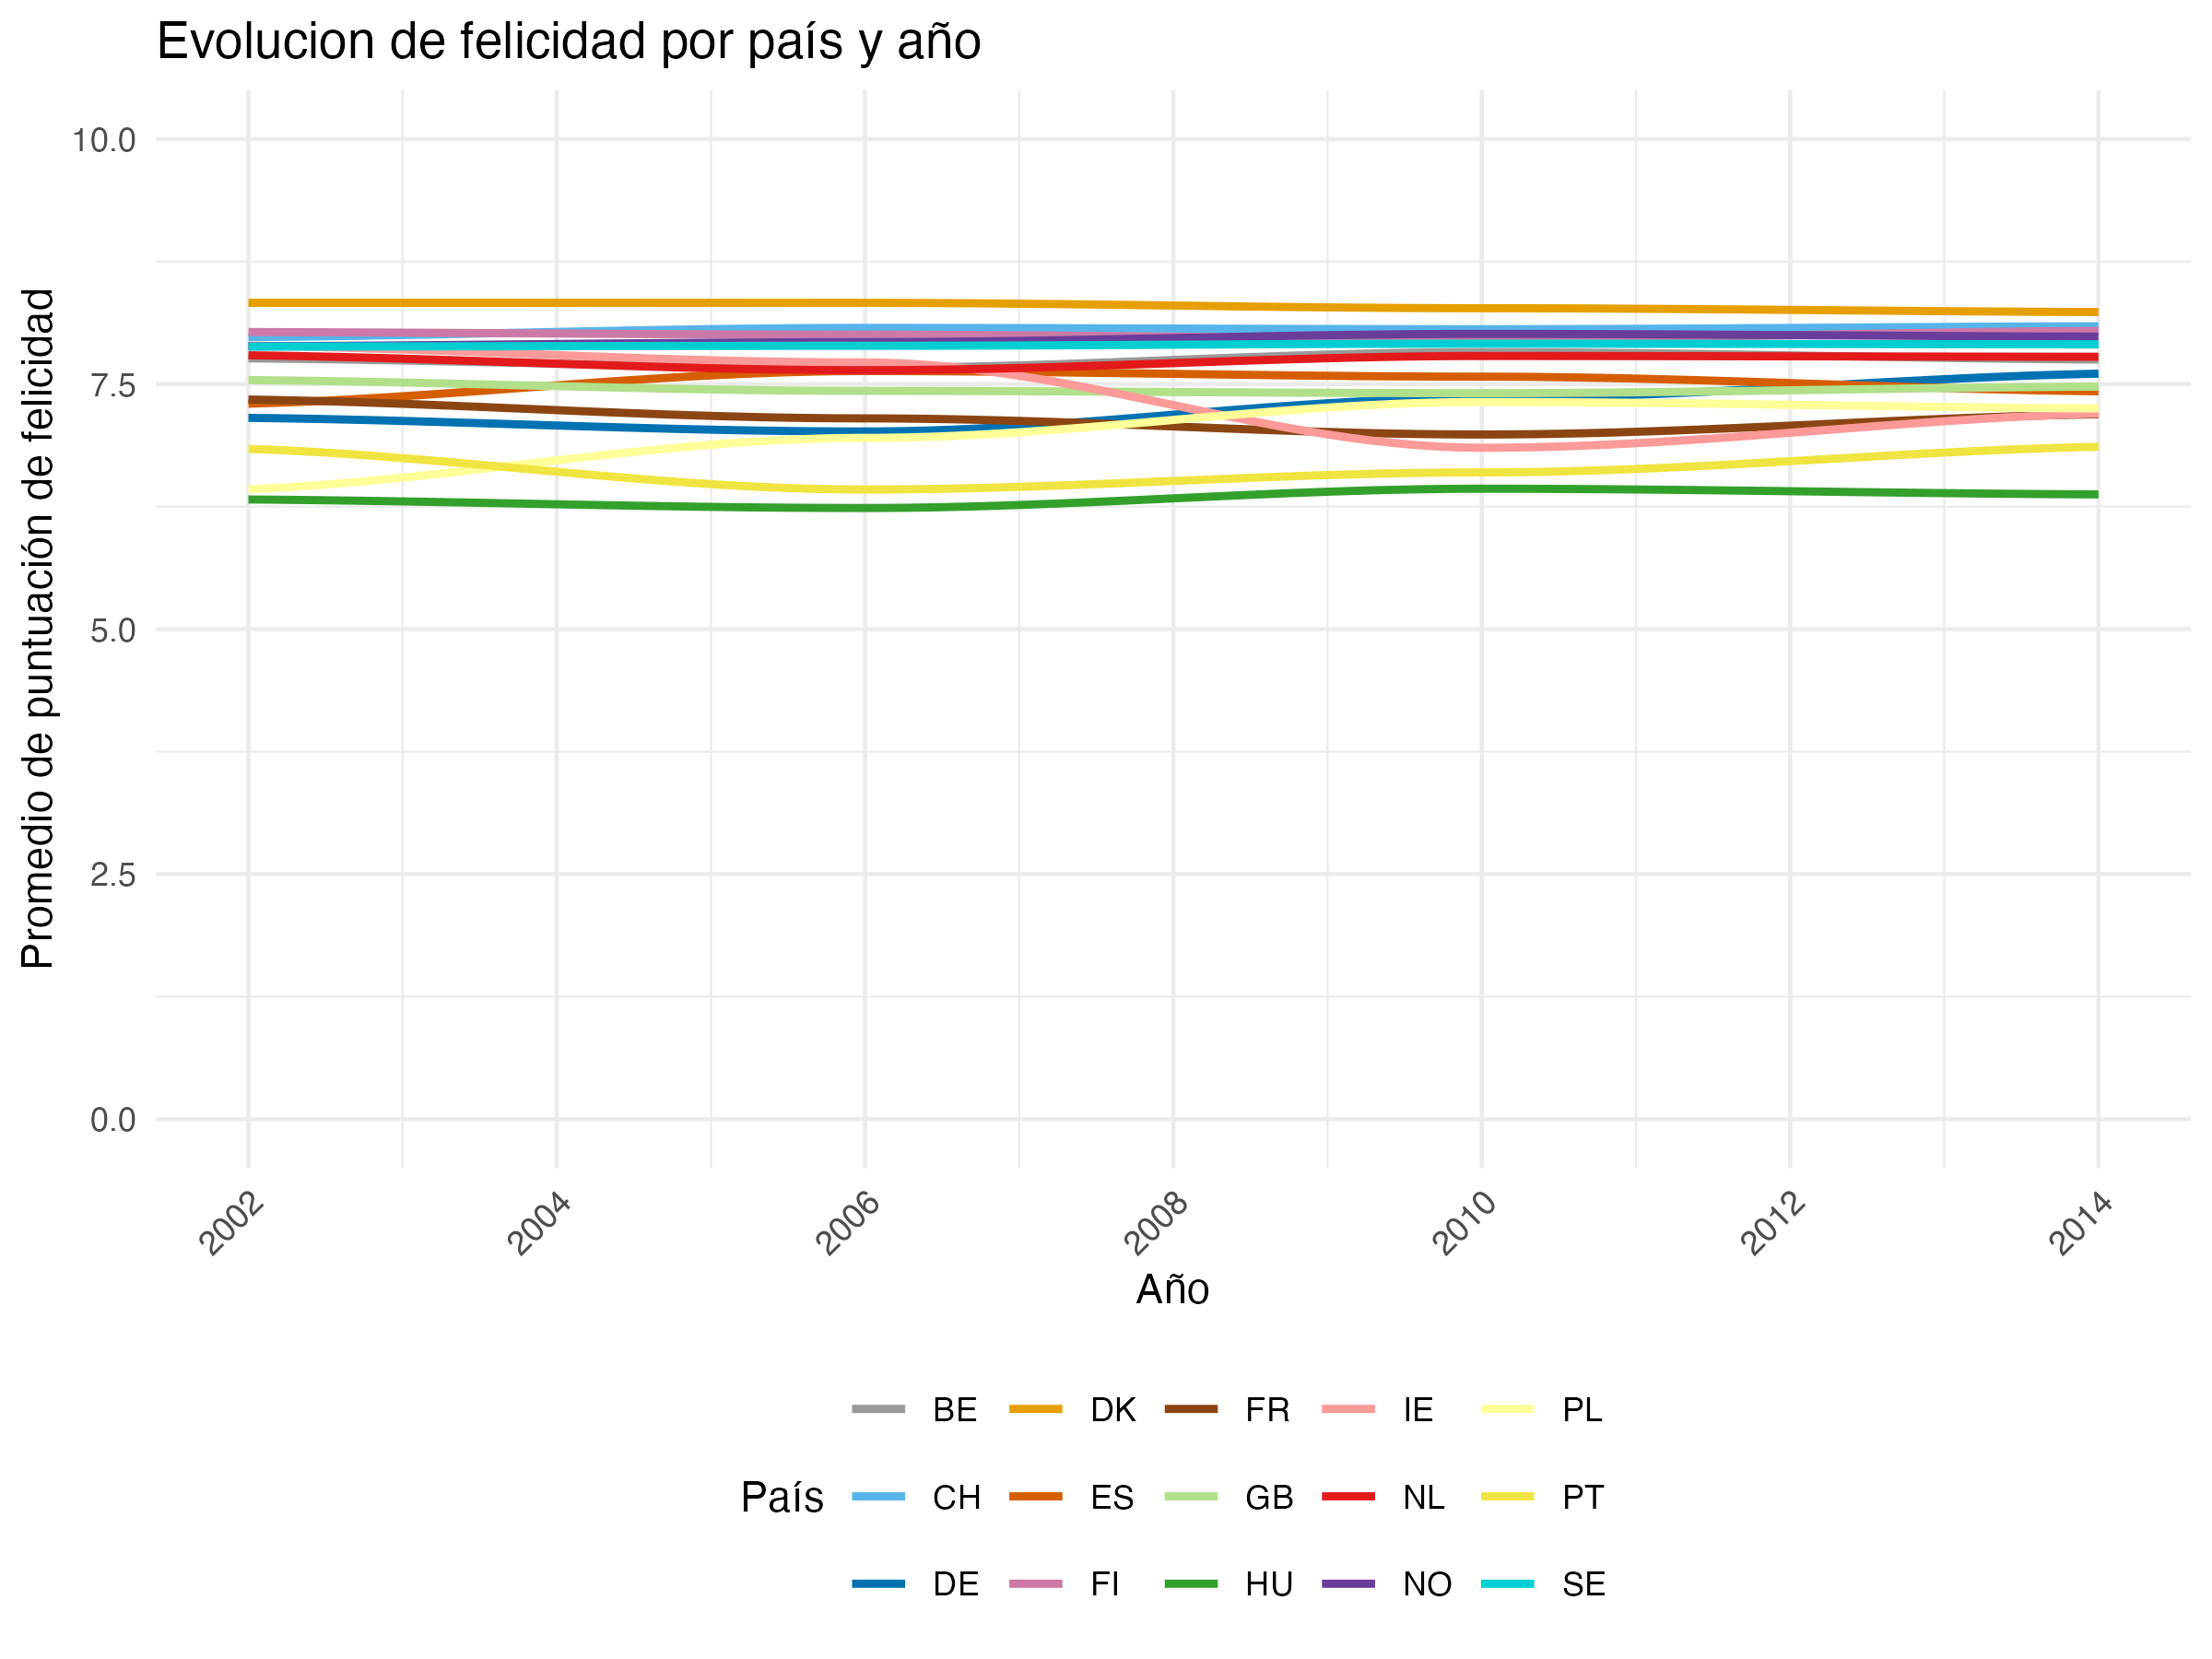
\includegraphics[scale=0.8]{grafico1.png}
\caption{Evolucion de felicidad por país y año}
\end{figure}

Podemos observar altos niveles de felicidad y una estabilidad media. 

\begin{figure}[h!]
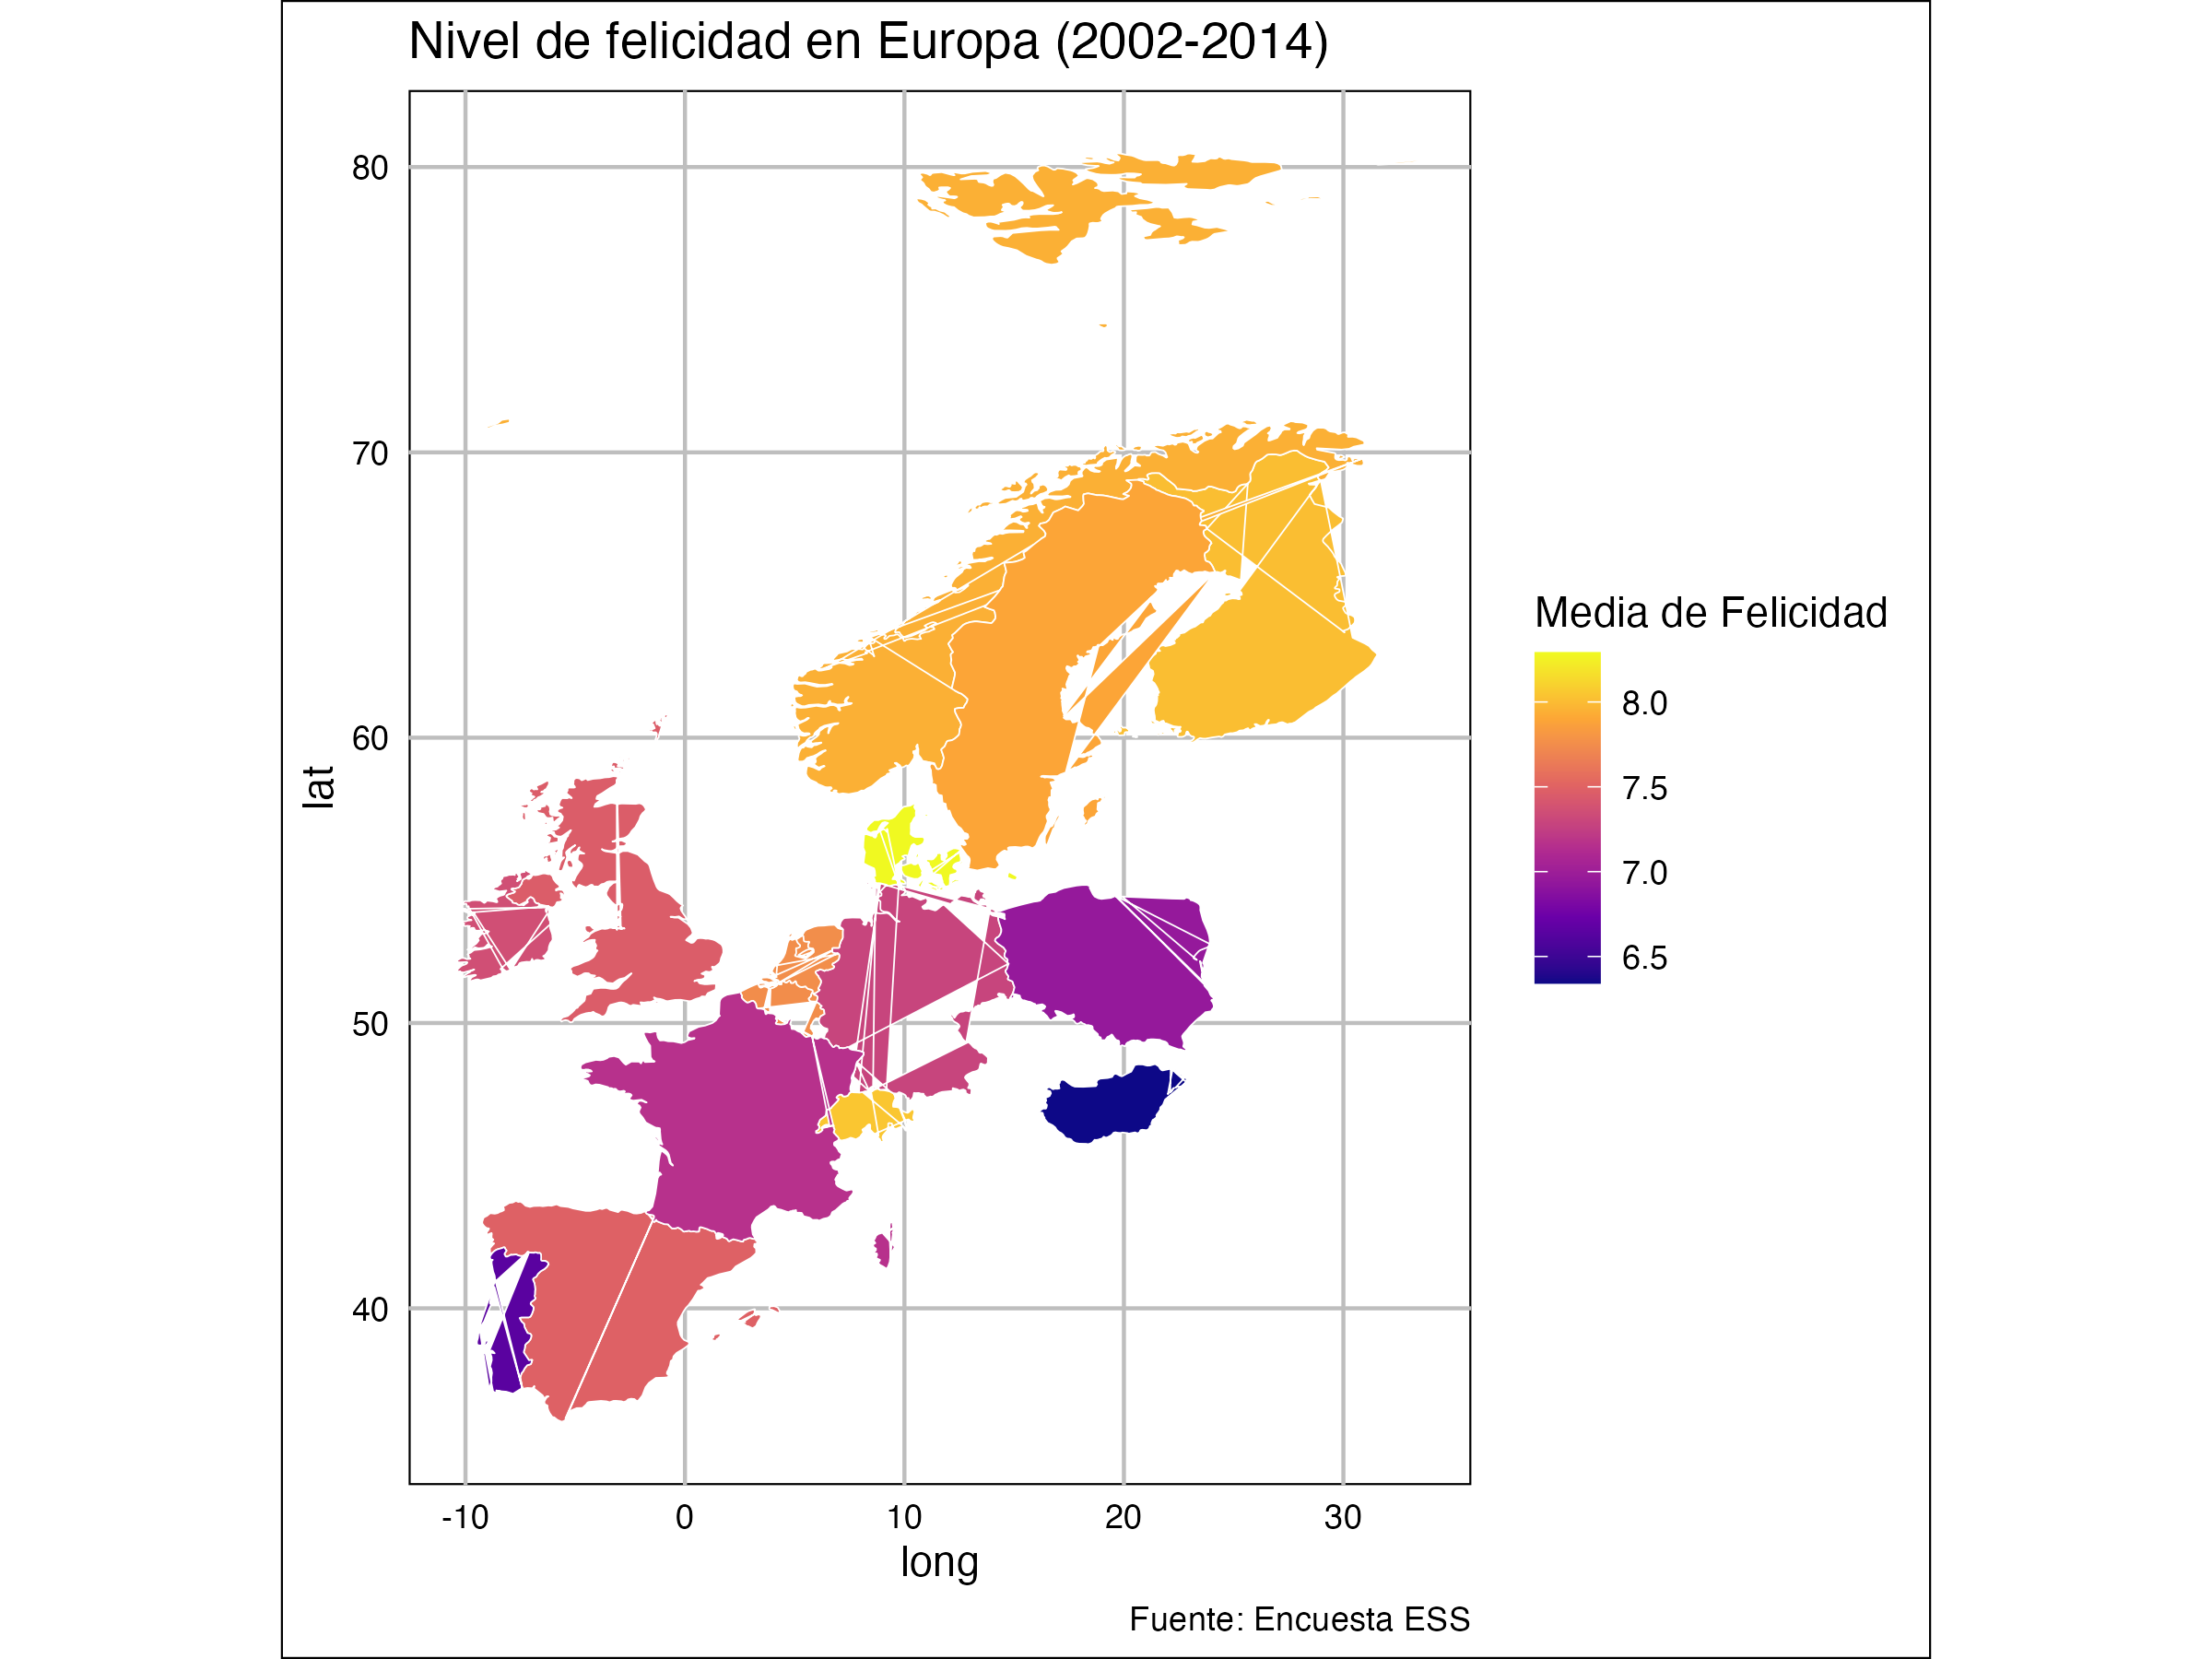
\includegraphics[scale=0.8]{grafico2.png}
\end{figure}



\begin{figure}[h!]
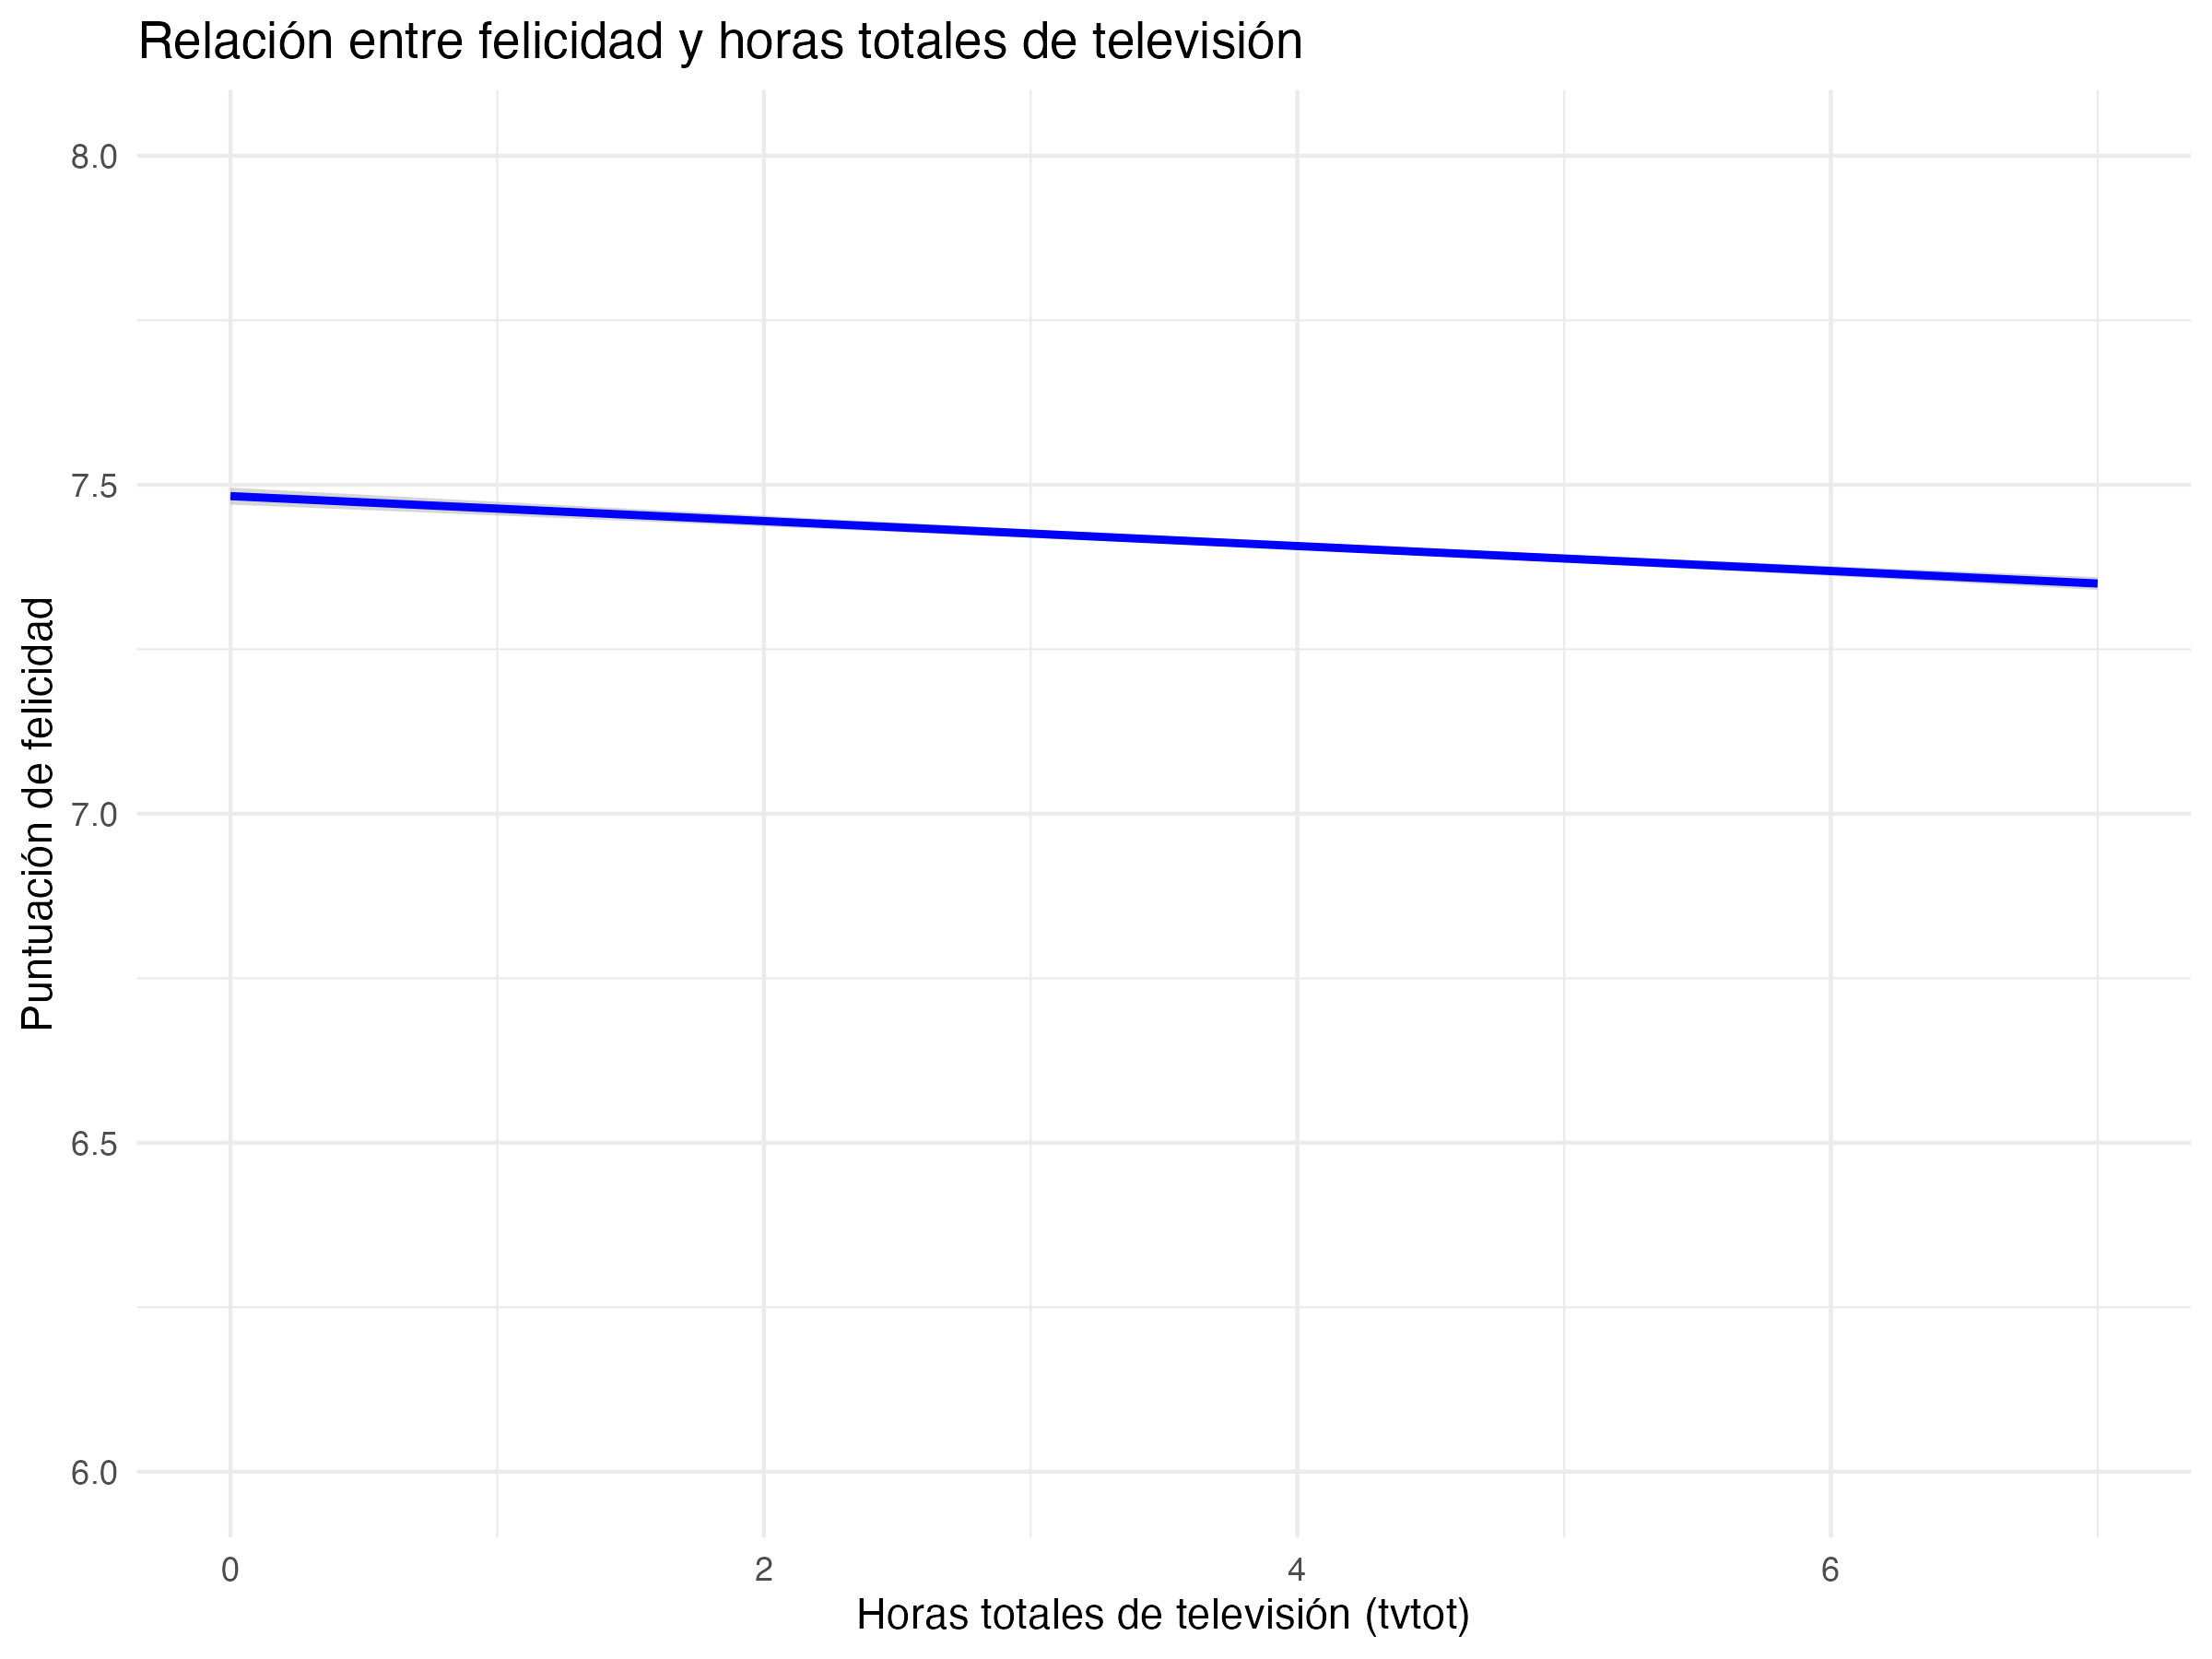
\includegraphics[scale=0.8]{grafico3.png}
\end{figure}

\begin{figure}[p]

Este gráfico permite observar cómo varía la felicidad en función del nivel de salud y el género, proporcionando una visión clara de la interacción entre estas variables.\\
\\
\\
\\
\\
\\
\centering 
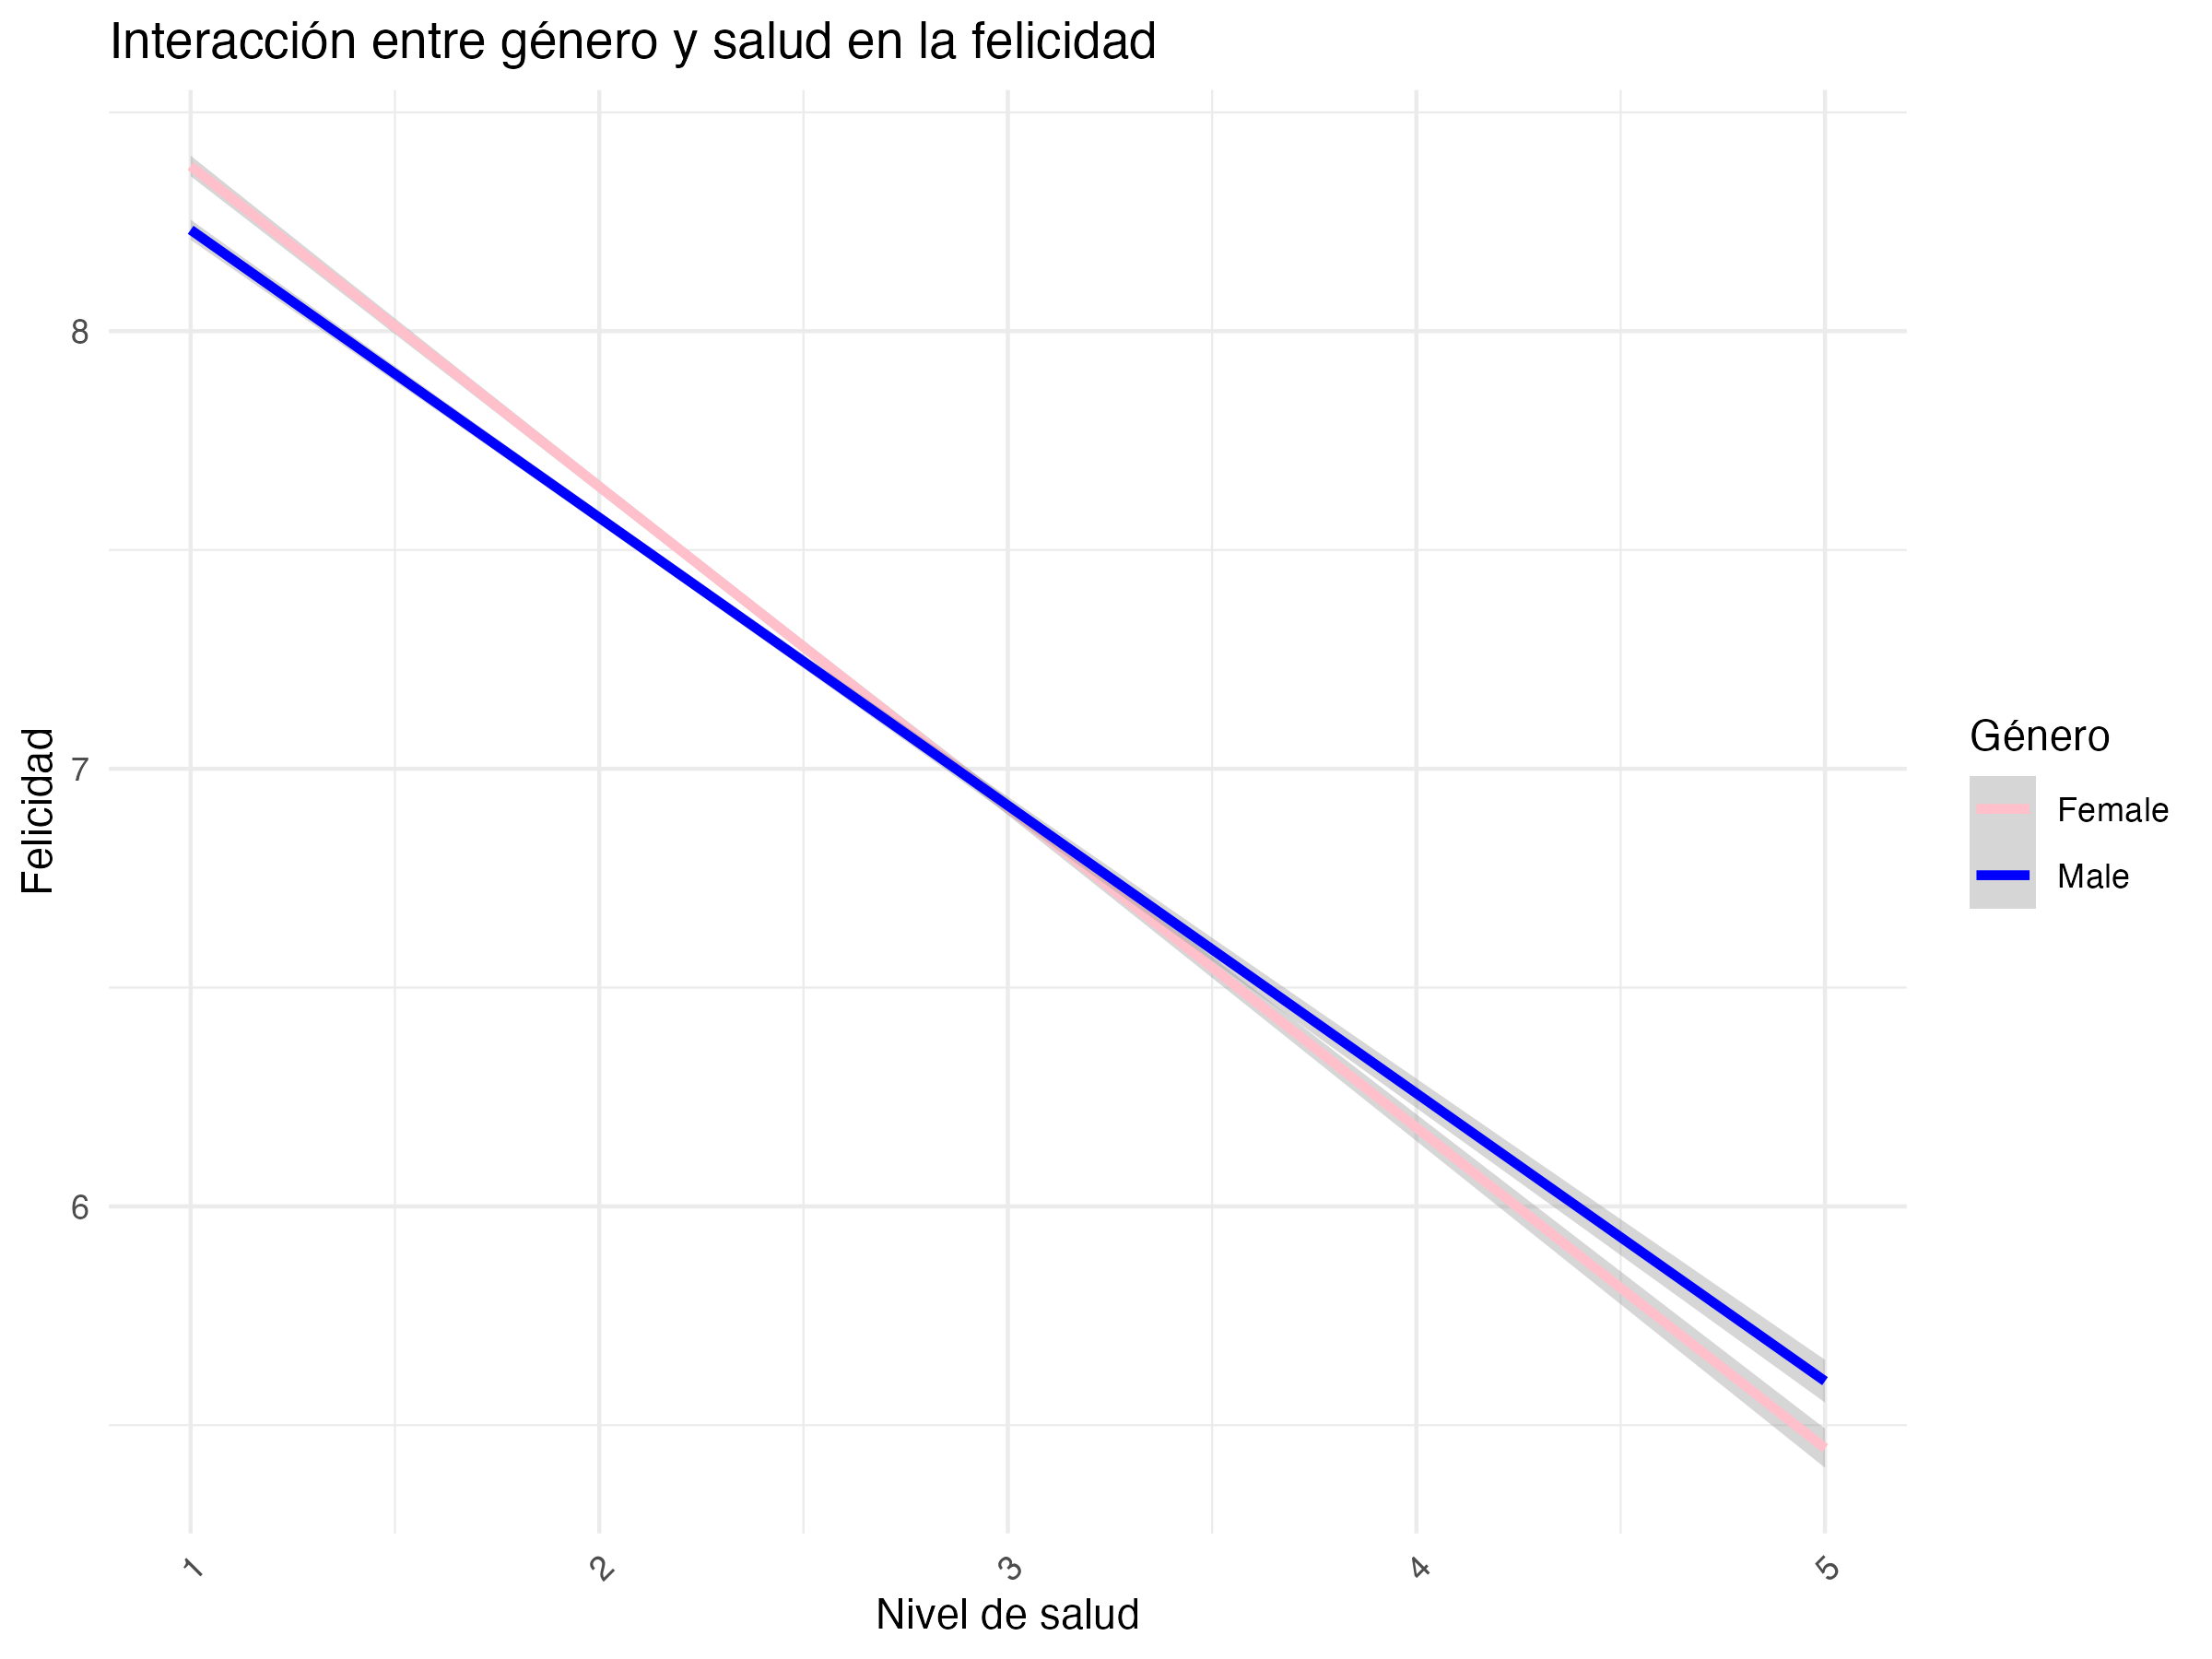
\includegraphics[scale=0.8]{grafico4.png}
\end{figure}


\clearpage % Forzar salto de página antes de la conclusión
\section {Conclusiones del análisis de datos y de la visualización de la felicidad europea (2002-2014)
}


El análisis de la felicidad en Europa entre los años 2002 y 2014, basado en los datos de 15 países seleccionados, revela varias observaciones interesantes a través de los cuatro gráficos presentados:

La visualización de la evolución temporal de la felicidad y de la media muestra que, en general, los niveles de felicidad se han mantenido relativamente estables en la mayoría de los países europeos durante el periodo estudiado. Sin embargo, destaca el hecho de que los países nórdicos, tradicionalmente considerados más fríos, como Dinamarca, Noruega y Suecia, muestran consistentemente altos niveles de felicidad en comparación con países más cálidos humanamente como España y Portugal. 

El gráfico de dispersión que analiza la relación entre la felicidad y el tiempo total de televisión revela una correlación muy baja entre estas variables. Esto indica que el tiempo dedicado a ver televisión no es un factor determinante en la percepción de felicidad de los individuos. 

El gráfico de interacción que muestra la relación entre felicidad, género y salud revela patrones interesantes que habría que estudiar. Aparentemente, existe una tendencia a que una mejor salud se asocie con menores niveles de felicidad, y viceversa. 

\end{document}
